\documentclass[12pt,a4paper]{report}
\usepackage{graphicx}
\usepackage[hungarian]{babel}
\usepackage[T1]{fontenc}
\usepackage[utf8]{inputenc}
\usepackage{multirow}
\usepackage{amsmath}
\usepackage{float}
\usepackage{enumerate}
\usepackage{caption}
\usepackage{setspace}
\usepackage{subcaption}
\usepackage{indentfirst}
\usepackage{color}
\usepackage{array}
\bibliographystyle{unsrt}
\usepackage[top=3cm ,bottom=3cm ,left=2cm ,right=2cm]{geometry}
\usepackage{multirow}
\usepackage{url}
\usepackage{listings}
\usepackage{color}
\begin{document}
\begin{titlepage}
	\centering
	{\scshape\LARGE Eötvös Loránd Tudományegyetem \par}
	\vspace{1cm}
	{\scshape\Large Kari Tudományos Diákköri dolgozat \par}
	\vspace{1.5cm}
	{\huge\bfseries A CBM/FAIR szimuláció használata és részecske klaszterezés nehézion ütközésekben\par}
	\vspace{2cm}
	{\Large\itshape Olar Alex - Fizika BSc III.\par}
	\vfill
	{\large Témavezető: Wolf György\par} 
	\begin{figure}[H]
	\centering
	\begin{subfigure}{.39\textwidth}
		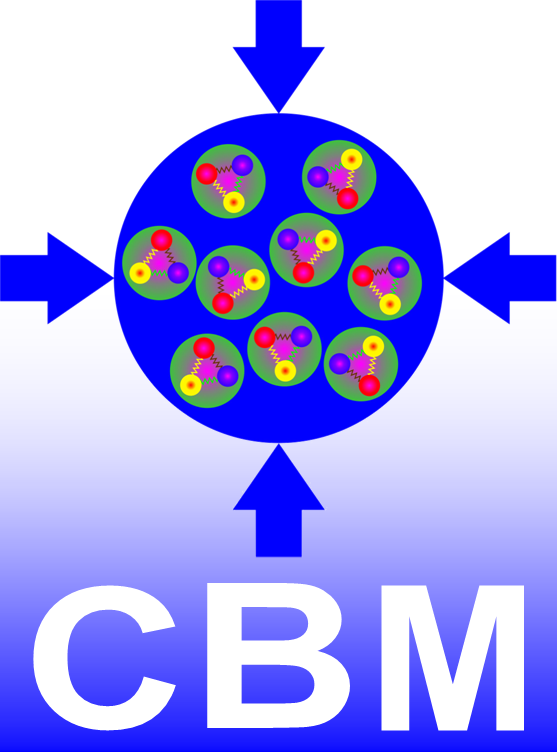
\includegraphics[width=0.82\textwidth]{gsi.png}
	\end{subfigure}
	\begin{subfigure}{.39\textwidth}
		
\includegraphics[width=.82\textwidth]{elte.jpg}
	\end{subfigure}
	\end{figure}
	\begin{figure}[H]
		\centering
		
\includegraphics[width=0.4\textwidth]{wigner.png}
	\end{figure}
	\vfill
\end{titlepage}
\end{document}